\section{Vision}


\begin{frame}{A Shared Vision}

\alert{TrustChain and Martel share a common vision} for a Web that
is
\begin{itemize}
    \item Human-centred
    \item Decentralised
    \item Trustworthy
    \item Privacy-preserving
    \item Open-source
\end{itemize}
where individuals, not big corporations, are truly in control of
their data.

\end{frame}


\begin{frame}{The Web Today}
  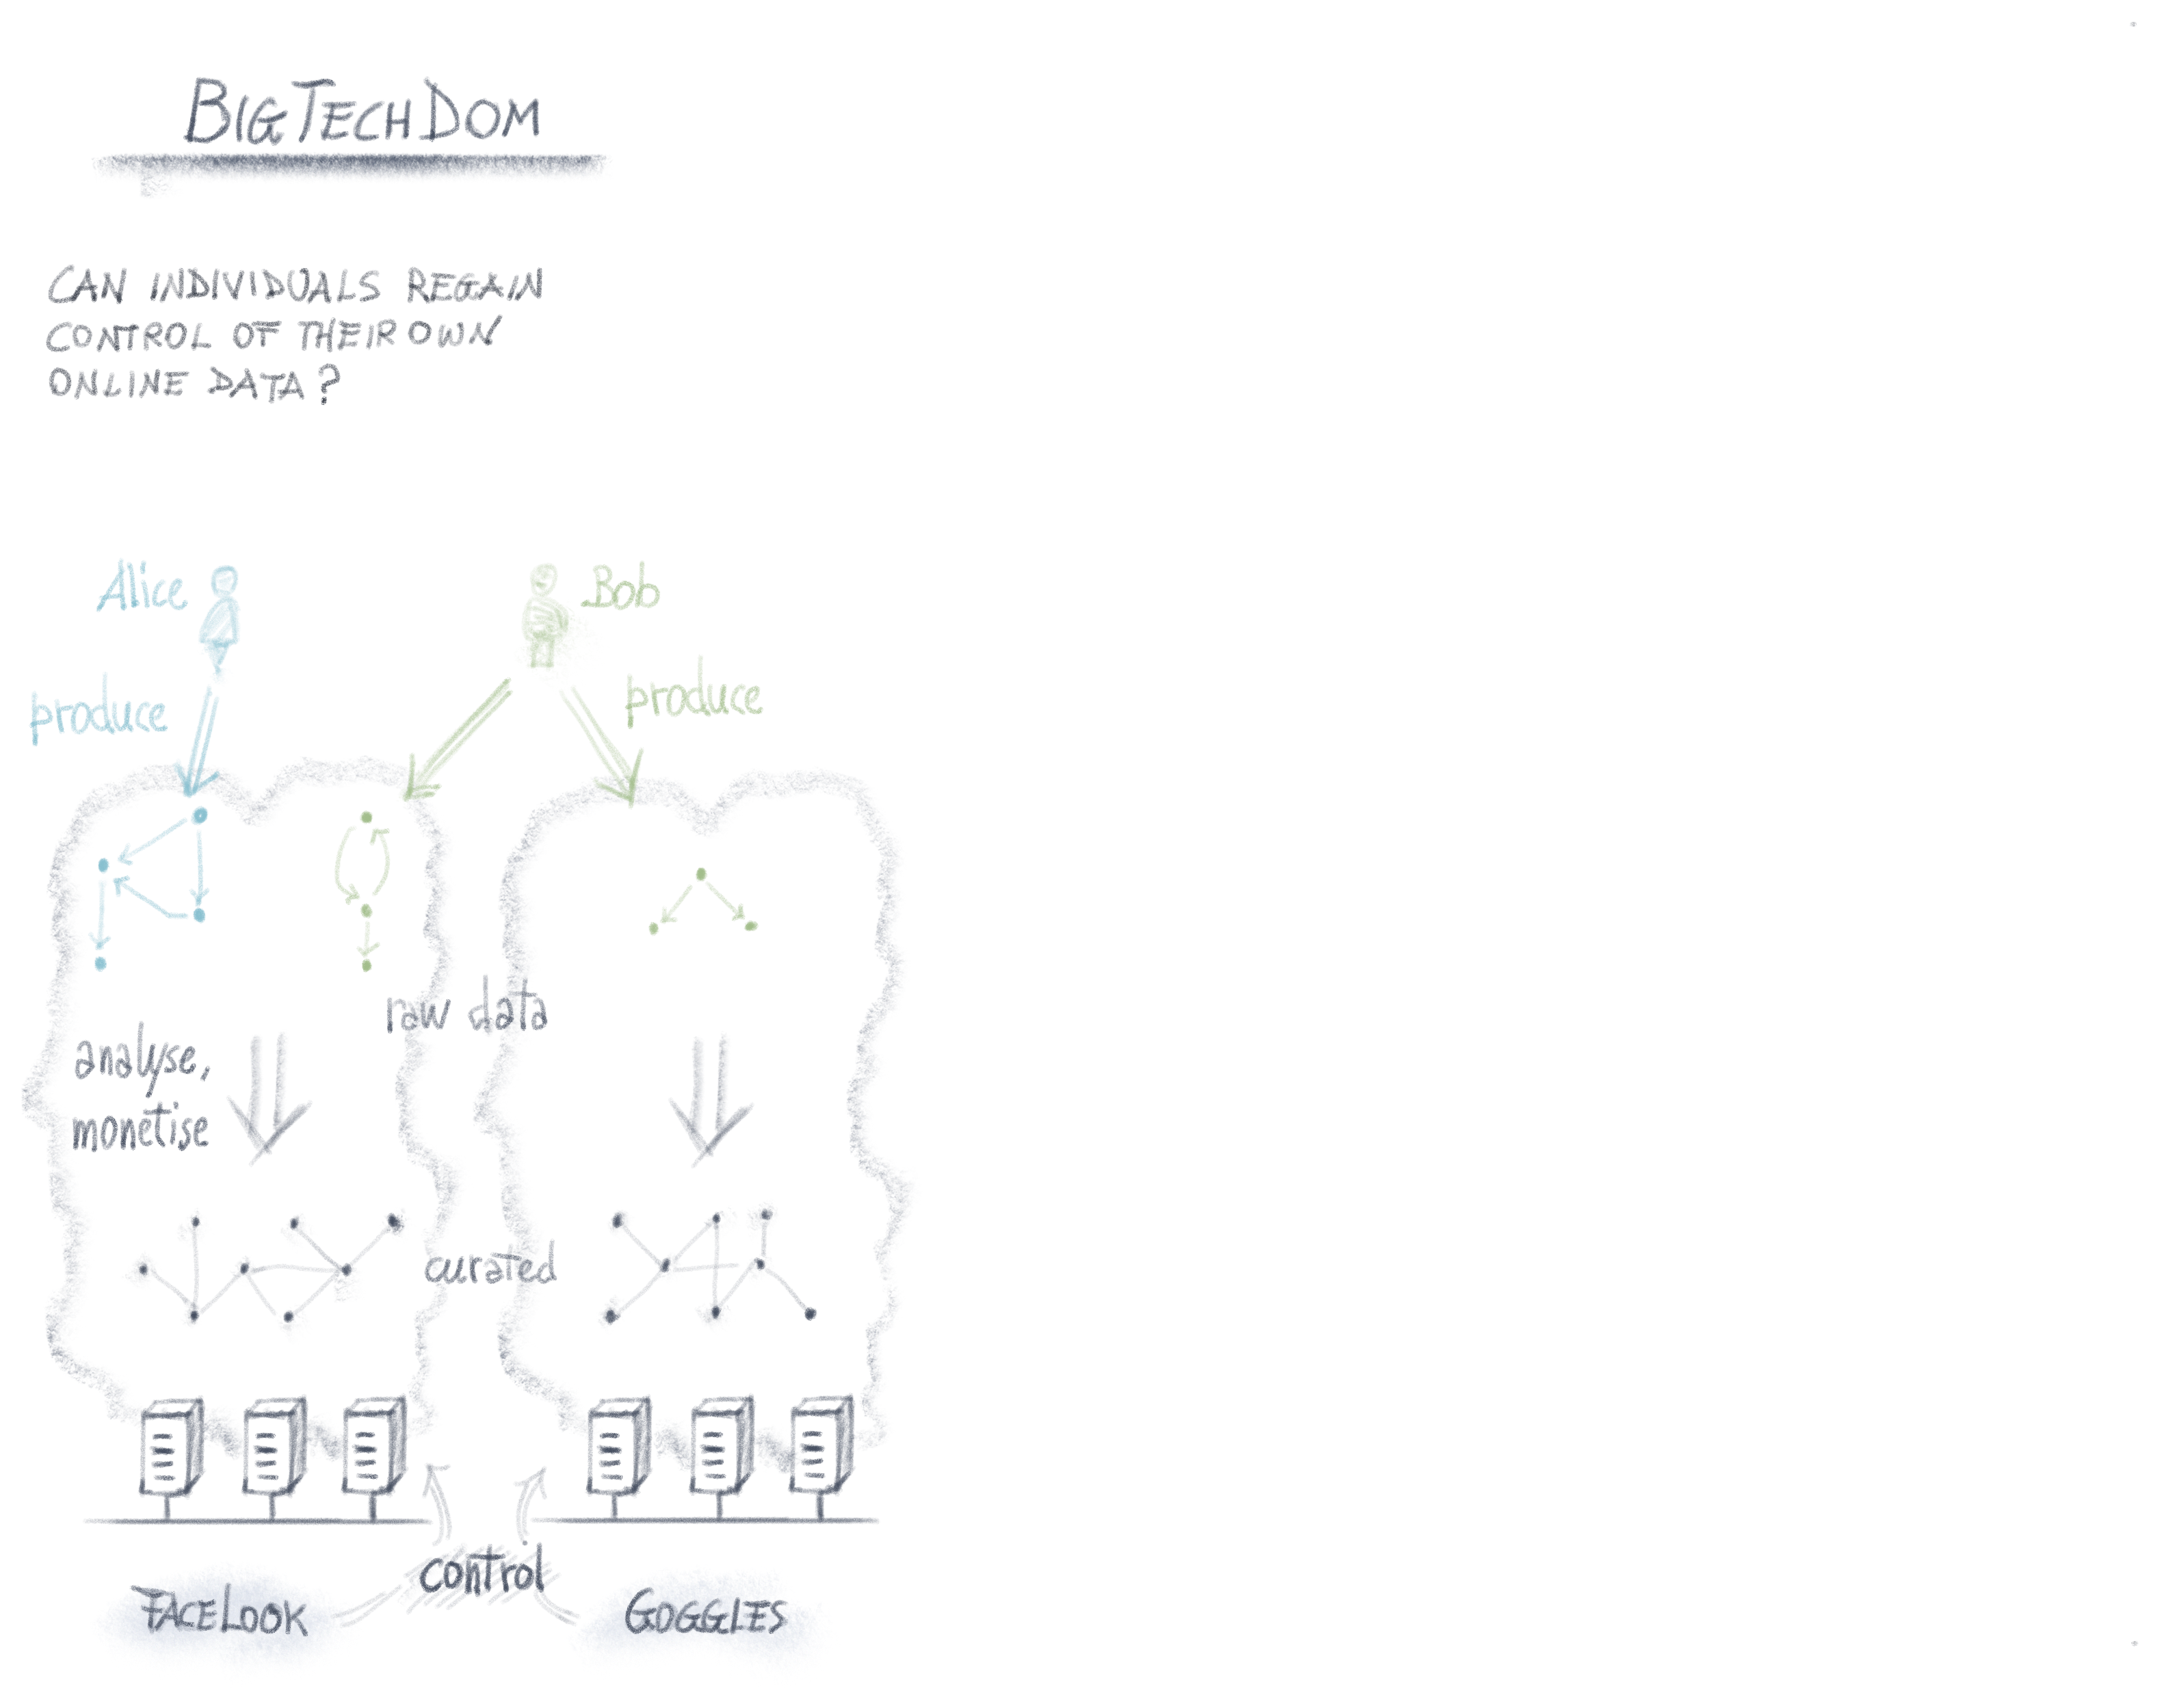
\includegraphics[height=0.85\paperheight]{./media/vision.1.png}
\end{frame}


\begin{frame}{The Web Tomorrow?}
  \includegraphics[height=0.85\paperheight]{./media/vision.2.png}
\end{frame}


\begin{frame}{The Snag}

A strong privacy and security architecture is critical to realise
this vision.

But how strong is the spec and how secure are WAC implementations
themselves?

\bigskip

IBM's 2023 data breach report:
\begin{itemize}
    \item Bugs cause 40\% of the data breaches
    \item Average data breach cost: \$4,000,000
\end{itemize}

\bigskip

So why should a user trust an implementation to be secure?

\end{frame}


\begin{frame}{Want}

For individuals to truly regain control of their online data in a
decentralised architecture, WAC implementations should provide
\begin{itemize}
  \item \alert{strong correctness guarantees}
\end{itemize}

But to check whether an implementation is correct, the spec must be
\begin{itemize}
  \item \alert{unambiguous}---exactly one interpretation exists
  \item \alert{consistent}---free of contradictions
\end{itemize}

\end{frame}


\begin{frame}{Mission}

Contribute to the Solid journey by improving \& extending WAC
\begin{itemize}
  \item Decentralised
  \item Provably secure
  \item Consistent
  \item User-friendly
\end{itemize}

\end{frame}
